 \documentclass[10pt,a4paper]{article}
\usepackage[utf8]{inputenc}
\usepackage[spanish]{babel}
\usepackage{pdfpages}
\usepackage[justification=centering]{caption}
\usepackage{textcomp}
\usepackage{gensymb}
\usepackage{fancyhdr}
\usepackage{amsmath}
\usepackage{alltt}
\usepackage{multirow}
\usepackage{epstopdf}
\usepackage{lastpage}
\usepackage{circuitikz}
\usetikzlibrary{arrows, decorations.markings}
\usepackage[pdfpagelabels,bookmarks,hyperindex,hyperfigures, hidelinks]{hyperref}

\tikzstyle{vecArrow} = [thick, decoration={markings,mark=at position
	1 with {\arrow[semithick]{open triangle 60}}},
double distance=1.4pt, shorten >= 5.5pt,
preaction = {decorate},
postaction = {draw,line width=1.4pt, white,shorten >= 4.5pt}]
\tikzstyle{innerWhite} = [semithick, white,line width=1.4pt, shorten >= 4.5pt]
\graphicspath{{assets/}}

\setcounter{MaxMatrixCols}{20}

\setlength{\headheight}{50pt}
\pagestyle{fancy}
\fancyheadoffset{0.5cm}
\fancyhead{}
\fancyhead[L]{
\includegraphics[scale=0.125]{FCEIA-logo.png}}
\fancyhead[C]{Universidad Nacional de Rosario\\Facultad de Ciencias Exactas, Ingeniería y Agrimensura\\Escuela de Ingeniería Electrónica}
\fancyhead[R]{
\includegraphics[scale=0.06]{LOGO-UNR-NEGRO.png}}

\renewcommand{\figurename}{Fig.}

\renewcommand\footrule{\begin{minipage}{1\textwidth}
	 \hrule width \hsize   
	\end{minipage}\par}

\setlength{\footskip}{0pt}
\fancyfoot[L]{\textit{Anteproyecto - F. Ceccarelli, M. Moya, L. Santos}}
\fancyfoot[C]{}
\fancyfoot[R]{\textit{Página \thepage{} de \pageref{LastPage}}}

\DeclareGraphicsExtensions{.bmp, .png, .jpg}

\renewcommand*\contentsname{Índice}

\topmargin = -1cm
\leftmargin = -1cm
\oddsidemargin = 0cm
\textheight = 24cm
\textwidth = 17cm

\begin{document}

\begin{titlepage}
\begin{minipage}{4cm}
\begin{flushright}

\includegraphics[scale=0.25]{FCEIA-logo.png}
\end{flushright}
\end{minipage}
\hfill
\begin{minipage}{4cm}
\begin{flushleft}

\includegraphics[scale=0.1]{LOGO-UNR-NEGRO.png}
\end{flushleft}
\end{minipage} \\ [10mm]
\begin{center}

 \large{ \textbf{Universidad Nacional de Rosario}} \\[5mm]
 \textbf{Facultad de Ciencias Exactas, Ingeniería y Agrimensura} \\[5mm]
 Escuela de Ingeniería Electrónica \\[20mm]
 \Large {\textbf{Área de Gestión de Proyectos}}\\[1.5mm]
 \small {Ingeniería Electrónica} \\[20mm]
 \Large {\textbf{Anteproyecto}} \\[5mm]
 \Large{ \textbf{Estudio e Implementación de un Sistema de Administración de Baterías de Li-Ion de baja y mediana potencia}} \\[15mm]

\end{center}
\begin{minipage}[t]{0.5\textwidth}
	{\large\textbf{Autores:}}
	\begin{itemize}
		\item Federico Ceccarelli (C-6241/3)
		\item Martin Moya (M-6132/8)
		\item Lucio Santos (S-4966/2)
	\end{itemize}
\vspace{10pt}
{\large\textbf{Directora:}}\\
\\
Dra. Monica Romero\\
\\
{\large\textbf{Asesor:}}\\
\\
Ing. Edgardo Arnejo


\end{minipage}
\begin{minipage}[t]{0.5\textwidth}
	\Large\textbf{Firma:}
\end{minipage}


\end{titlepage}

\tableofcontents

\clearpage

\section{Introducción}

\noindent A partir de la relevancia que ha comenzado a tomar el calentamiento global en las últimas décadas y el inquietante impacto que el mismo tiene sobre la calidad de vida de las personas, se han intentado buscar distintas soluciones para apaciguar las principales causas que generan un deterioro del medio ambiente, entre ellas, se encuentra el desarrollo de nuevas fuentes de energía renovables y su aprovechamiento.\\ 
\\
\noindent El vehículo eléctrico (VE) es considerado una de las transiciones tecnológicas más importantes de los últimos años debido a que no emiten dióxido de carbono ($\mathrm{CO_2}$) al medio ambiente y no utilizan combustibles fósiles para su funcionamiento, esto los convierte en uno de los avances tecnológicos más atractivos de los últimos tiempos teniendo en cuenta el avance del calentamiento global y el crecimiento del valor del petróleo.\\
\\
\noindent Siendo las baterías eléctricas la única fuente de energía en los VVEE, éstas tienen un gran impacto en la performance de los mismos determinando la autonomía del vehículo. En base a este criterio, las baterías de iones de litio (\emph{Li-Ion}) resultan las más adecuadas para esta aplicación debido a su alta densidad energética, es decir, que éste tipo de baterías tienen una gran capacidad para su reducido volumen a comparación de otras tecnologías. Para poder ser utilizados en VVEE, las baterías de Li-Ion son conectadas en forma de arreglos o packs de baterías en serie que permiten obtener mayores valores de tensión y, otras, en paralelo para aumentar la capacidad del pack. \\
\\
\noindent Sin embargo, a la hora de utilizar baterías de Li-Ion se debe tener en cuenta ciertos cuidados debido a que las mismas son propensas a fallar al ser sobrecargadas, completamente descargadas u operadas fuera del rango seguro de temperatura, lo que conlleva la implementación de un sistema de administración de baterías (\emph{BMS, por sus siglas en inglés Battery Management System}). Un BMS es un dispositivo encargado de controlar las funciones vitales de las baterías para que operen de forma correcta y segura con el objetivo de otorgar seguridad al usuario y prolongar la autonomía del vehículo. Las funciones más relevantes que llevan a cabo estos sistemas son:

\begin{itemize}
	\item Protección del pack para su operación en la región segura tanto en tensión, corriente como también en temperatura.
	\item Ecualización de las celdas individuales del pack, es decir, que la carga entre celdas sea uniforme.
	\item Estimación del estado de carga del pack de batería (\emph{SoC, por sus siglas en inglés State of Charge}).
	\item Estimación del estado de salud del pack de batería (\emph{SoH, por sus siglas en inglés State of Health}).
	\item Informar a la computadora central del vehículo los distintos parámetros del pack de baterías.
\end{itemize}

\noindent En un pack de baterías conectadas en serie, se pueden manifestar pequeñas diferencias de capacidades a través de todas las celdas, debido a tolerancias de producción o diferentes condiciones de operación, y tienden a incrementar con cada ciclo de carga. Además, las baterías sufren un proceso de \emph{auto-descarga} (típicamente entre un 2-10\% dependiendo de la temperatura y el estado de carga). Si la distribución de temperatura a lo largo del pack es heterogénea, las celdas con mayor temperatura tienden a una mayor pérdida de capacidad provocando un des balanceo de carga. Ésto trae varias consecuencias, entre ellas nos encontramos con:

\begin{itemize}
	\item \textbf{Seguridad:} Si el voltaje máximo de carga es excedido por unos cientos de milivoltios, puede provocar un embalamiento térmico, derritiendo el pack de baterias y, por lo tanto, el dispositivo que alimenta. En el peor de los casos puede explotar poniendo en riesgo el bienestar del usuario.
	\item \textbf{Salud de la batería:} La degradación de la batería es extremadamente sensible a la operación de la misma fuera de la zona indicada. Si la temperatura de operación o la tensión máxima de carga es excedida se provoca una aceleración en la degradación de su vida útil.
	\item \textbf{Carga incompleta:} Cuando el circuito de protección detecta que una de las celdas se encuentra cerca de condiciones inseguras de operación frena la carga del pack de baterías, en este caso nos encontramos con que una celda está completamente cargada y el resto no, obteniendo menos capacidad en el pack.
	\item \textbf{Autonomía:} Consideremos que el circuito de protección detecta que una de las baterías se encuentra descargada a niveles cercanos de operación insegura. En este caso, la protección frena la descarga del pack por una sola celda y el resto se encuentran con voltajes más altos y, por lo tanto, con un remanente de energía para entregar a la carga desaprovechando la capacidad del pack entero.
\end{itemize}


\clearpage

\section{Descripcion}

\subsection{Objetivos Generales}

\noindent Teniendo en cuenta las principales funcionalidades anteriormente descriptas, el objetivo de este proyecto es el desarrollo del hardware y el software de un Sistema de Administración de Baterías (\emph{BMS}) que cumpla con los siguientes requisitos, a saber.\\
\\
\noindent Proteger el pack de baterías evitando que el mismo salga de su zona de operación segura, tanto en tensión, corriente como en temperatura evaluando los umbrales correspondientes de operación para las celdas de Litio-Ion.\\
\\
\noindent Estimar el estado de carga en tiempo real utilizando estos datos con el fin de llevar al sistema al punto de operación óptima.\\
\\
\noindent Balancear la carga entre celdas priorizando el menor costo energético posible del sistema y la mayor autonomía final del pack.\\
\\
\noindent Comunicar los parámetros fundamentales del pack a una computadora central a través de algún protocolo estandarizado.\\
\\
\noindent Para lograr estos objetivos, se plantea un estudio pormenorizado del estado del arte de la temática en cuestión procurando seleccionar las prácticas y metodologías más adecuadas para la solución del problema planteado a partir de un estudio teórico. Finalmente se validará la solución elegida a partir de la implementación y ensayo de la solución desarrollada.

\subsection{Especificaciones}

El sistema a implementar  contará con los siguientes elementos:

\begin{itemize}
	\item \textbf{Pack de baterías} de arquitectura de hasta 6 celdas \emph{NCR18650} en serie.
	\item Sensado de tensión de las celdas individuales del pack y de la corriente que circula desde y hacia el pack de baterías.
	\item Etapa de potencia para el balanceo de las celdas.
	\item Protecciones encargadas de conectar y desconectar la carga del pack de baterías frente a operaciones fuera de la zona segura. 
	\item Microcontrolador basado en arquitectura ARM encargado de interconectar los distintos módulos del sistema, estimar el estado de carga y comunicar los parámetros del pack de baterías a la computadora central del vehículo.
\end{itemize}

\clearpage

\noindent La descripción anterior se puede visualizar en el Diagrama de Bloques (DB) de la Figura \ref{bms}
%(-1.2, 2.6) rectangle (5.2, -2.6);
% TODO: Modificar figura
\begin{figure}[h!]
	\begin{center}
		\begin{circuitikz}[european]
			\draw (-4, -1) rectangle (-2, 1)[fill=blue!10!white];
			\node at (-3, 0.2) {CPU};
			\node at (-3, -0.2) {Central};
			\draw [vecArrow] (-1.8, 0) to (-1, 0);
			\draw [vecArrow] (-1.2, 0) to (-2, 0);

			\draw (-1, -1) rectangle (1, 1)[fill=blue!10!white];
			\node at (0, 0) {MCU};
			
			\draw [blue,thin,dashed] (2.1, 2.5) rectangle (5.1, -2.5)[fill=blue!10!white];
			
			\draw (2.2, 2.4) rectangle (5.0, 0.92)[fill=yellow!15!white];
			\draw (2.2, 0.82) rectangle (5.0, -0.71)[fill=yellow!15!white];
			\draw (2.2, -0.81) rectangle (5.0, -2.4)[fill=yellow!15!white];
			

			
			\node at (3.6, 1.6) {Protección};			
			\node at (3.6, -1.6) {Equalización};
			\node at (3.6, 0) {Potencia};
			\draw [vecArrow] (1.2, 0) to (2.1, 0);
			\draw [vecArrow] (1.5, 0) to (1, 0);

			\draw (7, 2) -- (7, 2.2);
			\draw (7, 2) to[battery1] (7, 1.6);
			\draw (7, 1.4) -- (7, 1.6);
			\draw (7, 1.4) to[battery1] (7, .9);			
			\draw (7, .7) -- (7, .9);			
			\draw (7, 0.7) to[battery1] (7, 0.2);			
			\draw (7, 0.2) -- (7, -0.2);
			\draw (7, -0.2) to[battery1] (7, -0.7);
			\draw (7, -.7) -- (7, -.9);
			\draw (7, -.9) to[battery1] (7, -1.4);
			\draw (7, -1.4) -- (7, -1.6);
			\draw (7, -1.6) to[battery1] (7, -2);
			\draw (7, -2) -- (7, -2.2);
			
			\draw (9, 2) -- (9, 2.2);
			\draw (9, 2) to[battery1] (9, 1.6);
			\draw (9, 1.4) -- (9, 1.6);
			\draw (9, 1.4) to[battery1] (9, .9);			
			\draw (9, .7) -- (9, .9);			
			\draw (9, 0.7) to[battery1] (9, 0.2);			
			\draw (9, 0.2) -- (9, -0.2);
			\draw (9, -0.2) to[battery1] (9, -0.7);
			\draw (9, -.7) -- (9, -.9);
			\draw (9, -.9) to[battery1] (9, -1.4);
			\draw (9, -1.4) -- (9, -1.6);
			\draw (9, -1.6) to[battery1] (9, -2);
			\draw (9, -2) -- (9, -2.2);
			
			\draw (11, 2) -- (11, 2.2);
			\draw (11, 2) to[battery1] (11, 1.6);
			\draw (11, 1.4) -- (11, 1.6);
			\draw (11, 1.4) to[battery1] (11, .9);			
			\draw (11, .7) -- (11, .9);			
			\draw (11, 0.7) to[battery1] (11, 0.2);		
			\draw (11, 0.2) -- (11, -0.2);
			\draw (11, -0.2) to[battery1] (11, -0.7);
			\draw (11, -.7) -- (11, -.9);
			\draw (11, -.9) to[battery1] (11, -1.4);
			\draw (11, -1.4) -- (11, -1.6);
			\draw (11, -1.6) to[battery1] (11, -2);
			\draw (11, -2) -- (11, -2.2);
			
			
			\draw (5.1, 0) to[short, -*] (7, 0);
			\draw (7, 0) to[short, -*] (9, 0);
			\draw (9, 0) to[short, -*] (11, 0);
			
			\draw (7, 0.8) to[short, -*] (9, 0.8);
			\draw (9, 0.8) to[short, -*] (11, 0.8);
			
			\draw (7, 1.5) to[short, -*] (9, 1.5);
			\draw (9, 1.5) to[short, -*] (11, 1.5);
			
			\draw (7, 2.2) to[short, -*] (9, 2.2);
			\draw (9, 2.2) to[short, -*] (11, 2.2);			
			
			\draw (7, -0.8) to[short, -*] (9, -0.8);
			\draw (9, -0.8) to[short, -*] (11, -0.8);
			
			\draw (7, -1.5) to[short, -*] (9, -1.5);
			\draw (9, -1.5) to[short, -*] (11, -1.5);
			
			\draw (7, -2.2) to[short, -*] (9, -2.2);
			\draw (9, -2.2) to[short, -*] (11, -2.2);			
			
			\draw (5.1, 0.2) -- (6.2, 0.2) |- (7, 0.8) node at (7, .8){$\bullet$};
			\draw (5.1, 0.4) -- (6, 0.4) |- (7, 1.5) node at (7, 1.5){$\bullet$};
			\draw (5.1, 0.6) -- (5.8, 0.6) |- (7, 2.2) node at (7, 2.2){$\bullet$};
			
			\draw (5.1, -0.2) -- (6.2, -0.2) |- (7, -0.8) node at (7, -.8){$\bullet$};
			\draw (5.1, -0.4) -- (6, -0.4) |- (7, -1.5) node at (7, -1.5){$\bullet$};
			\draw (5.1, -0.6) -- (5.8, -0.6) |- (7, -2.2) node at (7, -2.2){$\bullet$};
			
			\draw [dashed] (-1.2, 2.6) rectangle (5.2, -2.6);
			\draw node at (-.8, 2.8){BMS};
			
			\draw [dashed] (6.5, 2.4) rectangle (11.5, -2.4);
			
			\draw node at (8.2, 2.6) {Pack de Baterías 6s3p};
			


			\draw (13, 1) to[R=$Z$] (13, -1);
			
			\draw (11, 2.2) -- (12, 2.2)
			|- (12, 1.5) -- (13, 1.5) |- (13,1) node at (12, 1.5){$\bullet$};
			
			\draw (11, -2.2) -- (12, -2.2)
			|- (12, -1.5) -- (13,-1.5) |- (13,-1) node at (12, -1.5){$\bullet$};
			
			
			
			\draw node at (12.8, 1){+};
			\draw node at (12.8, -1){-};
			
			
		\end{circuitikz}
	\end{center}
	\caption{Diagrama en Bloques del BMS y el pack de baterías}
	\label{bms}
\end{figure}


\noindent Para la prueba  de los distintos algoritmos y las protecciones del BMS, se plantea un esquema de realimentación \emph{(figs. \ref{realimentacion_esc} y \ref{realimentacion_cargador})} en donde el BMS se comunica con una computadora a través de un puerto que logre simular el protocolo estandarizado, obteniendo información del estado de carga del pack, la operación tanto del algoritmo de ecualización como las protecciones, voltaje y corriente de cada celda, a su vez, éste puede estar conectado a un banco de prueba, que puede estar compuesto por un inversor y un motor de alterna y/o continua, para evaluar el desempeño del algoritmo durante la descarga o conectado al cargador para ensayar el funcionamiento del mismo lo mismo ante una etapa de carga del pack de baterías.

%TODO: Modificar figuras
\begin{figure}[h!]
	\begin{center}
		\begin{circuitikz}
			\draw (-1,1) rectangle (1, -1) node at (0, 0) {PC};
			
			\draw [vecArrow] (1.2, 0) to (2, 0);
			\draw [vecArrow] (1.8, 0) to (1, 0);
			
			\draw (2,1) rectangle (4, -1) node at (3, 0) {BMS};
			
			\draw [vecArrow] (4, 0) to (5, 0);
			
			\draw (5,1) rectangle (7, -1) node at (6, 0.4) {Batería} node at (6, -.4) {6s3p};
			
			\draw (7, 0) -- (7.5,0)  |- (8, 0.1) node at (7.8, 0.4){+};
			\draw (3, -1) |- (7.5, -1.2) |- (8, -.1) node at (7.8, -0.4){-};
			
			\draw (8, 1) rectangle (10, -1) node at (9, 0.4) {ESC} 
			node at (9, 0) {+} node at (9, -.4) {BLDC};
		\end{circuitikz}
	\end{center}
	\caption{DB del esquema de realimentación conectado al ESC y el BLDC.}
	\label{realimentacion_esc}
\end{figure}

\begin{figure}[h!]
	\begin{center}
		\begin{circuitikz}
			\draw (-1,1) rectangle (1, -1) node at (0, 0) {PC};
			
			\draw [vecArrow] (1.2, 0) to (2, 0);
			\draw [vecArrow] (1.8, 0) to (1, 0);
			
			
			\draw (2,1) rectangle (4, -1) node at (3, 0) {BMS};
			
			\draw [vecArrow] (4, 0) to (5, 0);
			
			\draw (5,1) rectangle (7, -1) node at (6, 0.4) {Batería} node at (6, -.4) {6s3p};
			
			\draw (7, 0) -- (7.5,0)  |- (8, 0.1) node at (7.8, 0.4){+};
			\draw (3, -1) |- (7.5, -1.2) |- (8, -.1) node at (7.8, -0.4){-};
			
			\draw (8, 1) rectangle (10, -1)
			node at (9, 0) {Cargador};
		\end{circuitikz}
	\end{center}
	\caption{DB del esquema de realimentación conectado al ESC y el cargador del pack.}
	\label{realimentacion_cargador}
\end{figure}

\noindent Una vez finalizada esta etapa, solo resta probar los algoritmos sobre un EV (en este caso, una bicicleta) para validar la eficiencia de los mismos y elegir el más óptimo en base a la autonomía del vehículo. Finalizada la prueba, tenemos un sistema eficiente para implementar sobre vehículos eléctricos de baja y mediana potencia.

\clearpage

\section{Desarrollo}

\noindent Como se mencionó anteriormente, el BMS tendrá que cumplir una variedad de funcionalidades para poder monitorear y proteger el pack de baterías. A continuación, se detallan las especificaciones del pack y como se lograrán esos objetivos fundamentando, técnicamente, las metodologías y los recursos necesarios para llevar a cabo este proyecto.

\subsection{Batería de Litio-Ion}

\noindent Las baterías de Litio-ion son, hoy en día, una de las tecnologías, en almacenamiento de energía, más populares en el mundo debido a su uso en celulares, computadoras personales hasta en vehículos eléctricos. La comercialización de estas baterías comenzó en Japón en el año 1991, a diferencia de las baterías de ácido, que se vienen fabricando ya hace aproximadamente 150 años. Hay dos razones principales por las cuales las baterías de Litio-ion han crecido, en popularidad, en tan poco tiempo: su excelente rendimiento y la capacidad de adaptarse al creciente mercado de la electrónica de consumo, como por ejemplo, videograbadoras, celulares y computadoras. A partir de la primer década del siglo XXI, se comenzaron a utilizar en vehículos eléctricos, como también en grandes sistemas de almacenamiento de energía, capaces de alimentar barrios redicenciales enteros.\\
\\
\noindent Las baterías de litio-ion son definidas en \cite{def_liion} como almacenadores de energía que utilizan iones de Litio como portadores de carga. En base a esta definición, el término \emph{batería de Litio-Ion} no se corresponde con una sola composición química, como lo son las baterías de ácido o niquel-cadmio, si no que expresa una familia de baterías que dependen de los iones de Litio pero que pueden ser conformadas por distintos materiales.\\
\\
\noindent El principio de funcionamiento de las baterías de Litio se basa en que, durante el proceso de carga, el electrodo positivo (cátodo) libera iones de Litio al electrodo negativo (ánodo), y  en el proceso de descarga, el electrodo negativo provee al electrodo positivo Iones de Litio. La mayoría usan materiales de carbón, tales como el grafito y el carbón duro como ánodo, otros utlizan óxidos de metales, como por ejemplo, el Titanato de Litio ($\mathrm{Li_4Ti_5O_{12}}$) y el Pentóxido de Niobio ($\mathrm{Nb_2O_5}$), debido a que pueden aceptar iones de Litio cuando son cargados, y liberarlos en el proceso de descarga, estas reacciones se denominan como inserción y extracción respectivamente. Los potenciales de reacción de estos materiales son mucho más bajos que los electrodos de hidrógeno estándares, por lo tanto, el electrolito debería ser estable inclusive para niveles de potencial tan bajos. Ésta es la razón por la cual, los electrolitos orgánicos, que consisten de solventes orgánicos y sales de litio, son utilizados en las baterías de Litio-ion en vez de electrolitos acuosos.\\
\\
El material activo del cátodo debe contener Litio en su composición química para proveer una fuente de iones de Litio. Durante la primer etapa de desarrollo de las celdas de litio, se utilizaba Óxido de Litio-Cobalto ($\mathrm{LiCoO_2}$). También se estudió el uso de $\mathrm{LiNiO_2}$ como material activo para el cátodo pero fue inmediatamente descartado debido a su inestabilidad térmica. Sin embargo, se desarrollaron y utilizaron derivativos de esta composición, formulados como $\mathrm{LiM_xNi_{1-x}O_2}$ (M: elemento metálico tales como, el Co, Mn, Al, Mg).\\
\\
Las baterías de Litio-ion se destacan por las siguientes características:
\begin{itemize}
	\item \underline{Alto voltaje:} Las baterías de Li-ion tiene un voltaje típico entre 3 - 4V, debido al bajo potencial del ánodo.
	\item \underline{Alta energía específica:} Esto depende fuertemente del alto voltaje, porque la energía específica es el producto del voltaje de la celda y su capacidad específica, lo que hace que las celdas de Litio-Ion se destaquen a comparación de otras tecnologías, como por ejemplo, las celdas de Niquel-metal con un voltaje de 1.2V pero con mayor capacidad tienen menor energía específica. 
	\item \underline{Alta eficiencia energética:} Esto se debe a dos factores principales, por un lado se debe a la alta eficiencia de carga y descarga debido a que no hay pérdidas durante las reacciones químicas de la celda en ambos procesos y, nuevamente, esto se atribuye también a su alto voltaje. Éste último, se debe a que la eficiencia energética, es el restante de la tensión operativa en relación a la tensión en circuito abierto. Suponiendo que tenemos una celda A con una tensión de circuito abierto ($\mathrm{V_A}$) mayor que otra celda  B con una tensión $\mathrm{V_B}$, que tiene la misma pérdida de voltaje X, la eficiencia de A va a ser mayor que la de B, dado por:

\clearpage
	\begin{equation}
		\frac{V_A - X}{V_A} > \frac{V_B - X}{V_B} \nonumber
	\end{equation}
	\item \underline{Larga duración:} Esto se atribuye a que las reacciones dentro de la celda, durante los ciclos de carga y descarga, no realizan cambios morfológicos significativos. Esto es bastante distinto con las baterías de ácido, donde la reacción que se lleva a cabo involucra la disolución y deposición de materiales, lo que representa grandes cambios morfológicos durante los ciclos de carga y descarga.

\end{itemize}

\noindent Por último, las baterías de Litio-ion utilizan electrolitos orgánicos. El electrolito permite que la celda tenga alto niveles de tensión, sin embargo la combustibilidad del mismo genera problemas de seguridad. Por lo tanto, es clave para el desarrollo de estas baterías minimizar la causa y efecto de la combustión de la misma sin sacrificar rendimiento.\\
\\
\noindent El estado de las baterías de Litio-ion con respecto a las otras tecnologías se puede observar en la Figura \ref{comparisson}, donde se puede observar la dominancia de las mismas sobre el resto de las tecnologías, en términos de densidad energética (Wh/L) y energía específica (Wh/kg). La flecha de la esquina derecha indica que ésta tecnología se encuentra en constante desarrollo y puede mejorar con el paso del tiempo.\\
\\
\noindent Comercialmente, una sola celda consiste de dos electrodos (ánodo y cátodo), un separador entre ambos, una solución electrolítica dentro del separador, y un encapsulado que contiene todos los componentes mencionados anteriormente. Los electrodos son compuestos de cobre (ánodo) y aluminio (cátodo), revistiendolas por un material activo, un material conductivo, un aglutinante y un solvente, como por ejemplo, el N-Metil-2-Pirrolidona (NMP) o agua. El separador es un film microporoso de un polímero organíco, como por ejemplo, el polietileno, polipropileno, o un híbrido entre ambos.\\
\\
\noindent La aplicación práctica de las baterías de Litio-ion involucra la integración de las mismas dentro de un sistema, involucrando un controlador central (BMS), sistemas de refrigeración, sensores y conectores entre las celdas. En este sistemas las celdas pueden conectarse de distintas formas, por ejemplo, pueden conectarse en paralelo, para incrementar la capacidad del pack, en serie, para incrementar el voltaje, o combinadas para lograr ambos cometidos al mismo tiempo. Por ejemplo, un auto eléctrico de la marca \emph{Tesla}, posee un pack de baterías de 85KWh compuesto por 7104 celdas.\\
\\
\noindent En este caso utilizaremos celdas de Litio-ion modelo NCR18650, integrando una arquitecture \emph{6S3P}, es decir, por 6 celdas conectadas en serie y, cada celda de la cadena, es representada por 3 celdas en paralelo. En la Figura \ref{pack} se muestra el esquemático de la arquitectura del pack de baterías como también una foto de la celda que se utilizará para conformar el pack. 

\begin{figure}[h!]
		\begin{minipage}[c]{0.45\textwidth}
			\centering
			\begin{circuitikz}[european]

				\draw (7, 2) -- (7, 2.2);
				\draw (7, 2) to[battery1] (7, 1.6);
				\draw (7, 1.4) -- (7, 1.6);
				\draw (7, 1.4) to[battery1] (7, .9);			
				\draw (7, .7) -- (7, .9);			
				\draw (7, 0.7) to[battery1] (7, 0.2);			
				\draw (7, 0.2) -- (7, -0.2);
				\draw (7, -0.2) to[battery1] (7, -0.7);
				\draw (7, -.7) -- (7, -.9);
				\draw (7, -.9) to[battery1] (7, -1.4);
				\draw (7, -1.4) -- (7, -1.6);
				\draw (7, -1.6) to[battery1] (7, -2);
				\draw (7, -2) -- (7, -2.2);
				
				\draw (9, 2) -- (9, 2.2);
				\draw (9, 2) to[battery1] (9, 1.6);
				\draw (9, 1.4) -- (9, 1.6);
				\draw (9, 1.4) to[battery1] (9, .9);			
				\draw (9, .7) -- (9, .9);			
				\draw (9, 0.7) to[battery1] (9, 0.2);			
				\draw (9, 0.2) -- (9, -0.2);
				\draw (9, -0.2) to[battery1] (9, -0.7);
				\draw (9, -.7) -- (9, -.9);
				\draw (9, -.9) to[battery1] (9, -1.4);
				\draw (9, -1.4) -- (9, -1.6);
				\draw (9, -1.6) to[battery1] (9, -2);
				\draw (9, -2) -- (9, -2.2);
				
				\draw (11, 2) to[battery1] (11, 1.6);
				\draw (11, 1.4) -- (11, 1.6);
				\draw (11, 1.4) to[battery1] (11, .9);			
				\draw (11, .7) -- (11, .9);			
				\draw (11, 0.7) to[battery1] (11, 0.2);		
				\draw (11, 0.2) -- (11, -0.2);
				\draw (11, -0.2) to[battery1] (11, -0.7);
				\draw (11, -.7) -- (11, -.9);
				\draw (11, -.9) to[battery1] (11, -1.4);
				\draw (11, -1.4) -- (11, -1.6);
				\draw (11, -1.6) to[battery1] (11, -2);
				\draw (11, -2) -- (11, -2.2);
				
				\draw (7, 0) -- (9, 0);
				\draw (9, 0) -- (11, 0);
				
				\draw (7, 0.8) -- (9, 0.8);
				\draw (9, 0.8) -- (11, 0.8);
				
				\draw (7, 1.5) -- (9, 1.5);
				\draw (9, 1.5) -- (11, 1.5);
				
				\draw (7, 2.2) -- (9, 2.2);
				\draw (9, 2.2) -- (11, 2.2);			
				
				\draw (7, -0.8) -- (9, -0.8);
				\draw (9, -0.8) -- (11, -0.8);
				
				\draw (7, -1.5) -- (9, -1.5);
				\draw (9, -1.5) -- (11, -1.5);
				
				\draw (7, -2.2) -- (9, -2.2);
				\draw (9, -2.2) -- (11, -2.2);			
				
				\draw [dashed] (6.5, 2.4) rectangle (11.5, -2.4);
				
				\draw node at (8.2, 2.6) {Pack de Baterías 6s3p};
			\end{circuitikz}
		\end{minipage}
		\begin{minipage}[c]{0.45\textwidth}
			\centering
			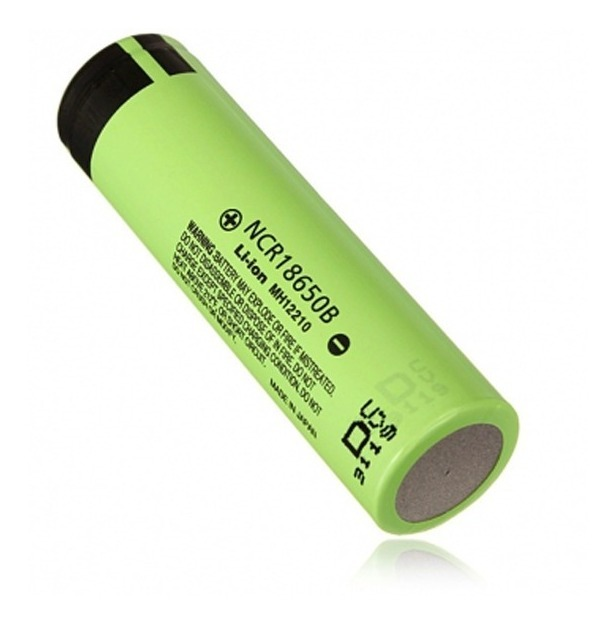
\includegraphics[width=0.45\textwidth]{18650.jpg}
		\end{minipage}
	\caption{A la izquierda se visualiza el esquemático de la arquitectura del pack de baterías. A la derecha se muestra una foto de una celda NCR18650B.}
	\label{pack}
\end{figure}

\clearpage

\subsubsection{NCR18650B}

En este caso, se opta por utilizar las baterías comerciales denominadas NCR18650B. Estas celdas se caracterizan por su cátodo, cuya composición química se basa en el óxido de Litio Niquel Cobalto Aluminio ($\mathrm{LiNiCoAlO_2}$) y, según su hojas de datos, sus propiedades generales se pueden observar en la Tabla \ref{ncr_table}.

\begin{table}[h!]
\begin{center}
\begin{tabular}{|c|l|}
\hline
\multicolumn{2}{|c|}{Especificaciones}                                             \\ \hline
\textbf{Capacidad Específica}                 & 3200mAh                            \\ \hline
\multirow{2}{*}{\textbf{Capacidad}}           & Mínimo: 3250mAh                    \\ \cline{2-2} 
                                              & Tipico: 3350mAh                    \\ \hline
\textbf{Corriente de Descarga Máxima}         & 4875mAh ($\sim$1.5C)               \\ \hline
\textbf{Rango operativo de tensión}           & 2.5V - 4.2V                        \\ \hline
\textbf{Voltaje Nominal}                      & 3.6V                               \\ \hline
\textbf{Charga}                               & CC-CV, Std. 1625mA, 4.20V, 4.0 hrs \\ \hline
\textbf{Peso}                                 & 48.5g                              \\ \hline
\multirow{3}{*}{\textbf{Temperatura}}         & Carga: 0 a 45C                     \\ \cline{2-2} 
                                              & Descarga: -20 a 65C                \\ \cline{2-2} 
                                              & Almacenaje: -20 a 50C              \\ \hline
\multirow{2}{*}{\textbf{Densidad Energética}} & Volumetrica: 676Wh/l               \\ \cline{2-2} 
                                              & Gravimetrica: 243wh/kg             \\ \hline
\end{tabular}%
\end{center}
\end{table}

Por el otro lado, la hoja de datos también nos provee curvas significativas, como por ejemplo, la curva de carga \emph{(Fig. \ref{cc_cv})}, la curva de descarga para distintas corrientes \emph{(Fig. \ref{descarga_18650})} y la curva del ciclo de vida típico de la batería \emph{(Fig. \ref{life_cycle_18650})}.

\begin{figure}[h!]
	\begin{center}
	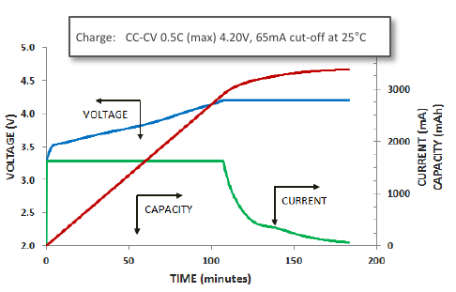
\includegraphics[width=0.7\textwidth]{cc_cv_18650.png}
	\caption{Curva de carga.}
	\label{cc_cv}
	\end{center}
\end{figure}

\begin{figure}[h!]
	\begin{center}
	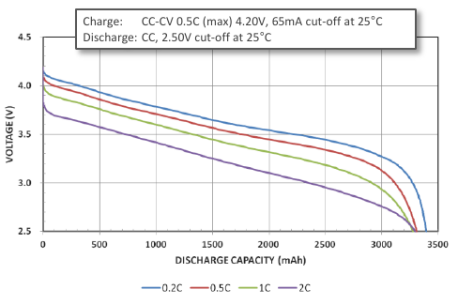
\includegraphics[width=0.7\textwidth]{discharge_18650.png}
	\caption{Curva de descarga en base a distintas corrientes de descarga (0.5C, 1C, 1.5C y 2C)}
	\label{descarga_18650}
	\end{center}
\end{figure}

\begin{figure}[h!]
	\begin{center}
	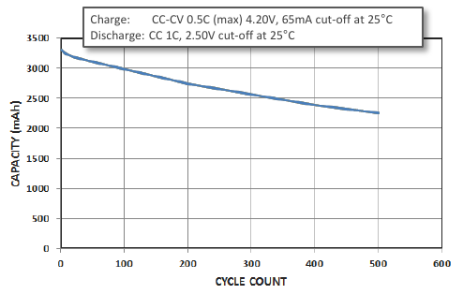
\includegraphics[width=0.7\textwidth]{life_cycle_18650.png}
	\caption{Curva del ciclo de vida de una celda 18650}
	\label{life_cycle_18650}
	\end{center}
\end{figure}

\clearpage

\subsection{Algoritmos de Estimación del Estado de Carga}
La estimación del estado de carga es una de las tareas fundamentales dentro del sistema de Administración de baterías ya que en base a esta información se toman importantes decisiones, de ella dependen la optima ecualización de carga de las celdas, no exceder los límites de Zona de Operación segura, realizar acciones preventivas en caso del agotamiento de carga como ser iniciar un apagado de seguridad y por último reportar al usuario la carga restante en el pack.\\

A priori hay 2 métodos básicos de estimación de carga, el primero aprovecha la relación entre el SOC y el OCV este método es económico pero tiene 2 principales desventajas, la curva OCV vs SOC tiene una región en la cual tiene valores de pendiente despreciable lo que genera que entre el 80\% de carga y el 35\% aproximadamente, haya solo unas pocas decenas de milivoltios de diferencia. Debido a esto un error de pocos milivolts genera grandes diferencias en la estimación de la carga real. Por otro lado la estimación mediante voltaje tiene problemas a la hora de determinar el voltaje online, es decir cuando la batería esta conectada a una carga las corrientes que circulan por el pack generan caidas de tensión debido a las impedancias internas del pack, si estas no son tenidas en cuenta pueden llevar a que el ecualizador del pack desbalancee aún más el pack.\\

El segundo método es el \textbf{\emph{Conteo de carga}} o \textbf{\emph{Coulomb Counting}}, el mismo consiste en integrar la corriente a lo largo del tiempo obteniendo así la carga total en el pack o SOC mediante la ecuación \ref{SOC_Coulomb_C}, donde \emph{i} corresponde a la corriente de la batería y $C_\eta$ la capacidad nominal de la misma.\\

\begin{figure}[h!]
	\begin{center}
		\begin{equation}
			SOC=1-\frac{\int{i.dt}}{C_\eta}\label{SOC_Coulomb_C}
		\end{equation}	
	\end{center}
\end{figure}

 Este método funciona muy bien en la zona donde el primer método falla, sin embargo como todo proceso de integración, genera errores iterativos en cada ciclo de cálculo generando que a lo largo del tiempo el error absoluto de este método tienda a crecer.Además de la necesidad de establecer un valor inicial de carga, estos puntos de referencia pueden ser la carga total de la batería o la máxima DOD de manera que exigen a la batería llegar a puntos límites de carga disminuyendo su vida útil.\\

Debido a que nos interesa saber el SOC cuando la batería esta entregando energía o siendo cargada se deben tener en cuenta los principales factores que afectan a la estimación de carga on-line. Un modelo utilizado para relacionar la tensión entre los bornes de la batería y el OCV utilizado con gran frecuencia es el modelo eléctrico bosquejado en la \emph{Fig. \ref{Electric_model}}, este modelo es coherente con el hecho de que la tensión en los bornes de la batería en reposo es igual al OCV. Pero al ser circulada por una corriente se deben tener en cuenta los fenómenos dinámicos  y la perdida por resistencias internas así como la corriente de pérdida (auto descarga) de la batería.
  
\begin{figure}[h!]
	\begin{center}
		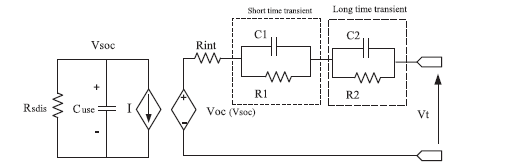
\includegraphics[width=0.7\textwidth]{electric_battery_model_2_order.png}
		\caption{Modelo Electrico de segundo orden con corriente de perdida.}
		\label{Electric_model}
	\end{center}
\end{figure}
Dada la naturaleza química de la batería, si se entra en detalle se puede observar que los componentes que modelan la batería tienen un comportamiento no lineal dependiendo del SOC y más aún se ven afectados por el efecto de envejecimiento de las celdas, es decir, estamos es un sistema no lineal no estacionario.
\clearpage
Como soluciones parciales fueron desarrollados varios métodos los cuales son una solución de compromiso entre aproximaciones lo suficientemente conservadoras para obtener el menor error posible y un alto costo computacional cuyas exigencias de hardware elevan el costo y el espacio necesario para su implementación, clasificándose según \cite{metodos_convencionales} los siguientes métodos como convencionales :\\
% \cite{metodos_convencionales}
%A review of lithium-ion battery state of charge estimation and management
%system in electric vehicle applications: Challenges and recommendations
%M.A. Hannan,⁎, M.S.H. Lipu, A. Hussain, A. Mohamed 
%el archivo se llama Lithium_SOC en la carpeta de papers
\begin{itemize}
	\item Fuerza Electro-Motriz
	\item Estimación basada en modelos (Térmico y electroquímicos)
	\item Resistencia interna
	\item Espectroscopia Dieléctrica
\end{itemize}

Un gran avance en la estimación del estado de carga fue la aplicación de los Filtro de Kalman para disminuir el error. Esta es una herramienta estadística de análisis en espacio de estado que mediante las matrices de Varianza y Covarianza estiman un vector de soluciones con mayor precisión. 
Los Filtros de Kalman ven afectado su rendimiento a la hora de trabajar con sistemas fuertemente No Lineales, debido a esto surgen las variantes EKF, UKF y SPKF provenientes del inglés, Extended, Unscented y Sigma Point, respectivamente.\\

\subsubsection{Método de estimación por FEM}
Teniendo en cuenta la limitación del método de OCV para la estimación mientras la batería esta siendo cargada o descargada, surge como solución a esta problemática la estimación del OCV mediante el estudio de la respuesta temporal de la tensión entre los terminales de la batería dado su comportamiento temporal regido por una ecuación diferencial de primer orden como se muestra en \emph{\ref{1er_orden_eq}}, siendo k una constante, cuya solución es de la forma \emph{\ref{1er_orden_sol}}, lo cual se corresponde con la gráfica de la \emph{Fig.\ref{EMF_Method}}.

\begin{figure}[h!]
	\begin{center}
		\begin{equation}
		\frac{df(x)}{dx} = \alpha f(x)
		\label{1er_orden_eq}
		\end{equation}	
	\end{center}
\end{figure}

\begin{figure}[h!]
	\begin{center}
		\begin{equation}
		f(x)= x_{(\infty)}+(x_0-x_{(\infty)})e^{-\alpha x}
		\label{1er_orden_sol}
		\end{equation}	
	\end{center}
\end{figure}

\begin{figure}[h!]
	\begin{center}
		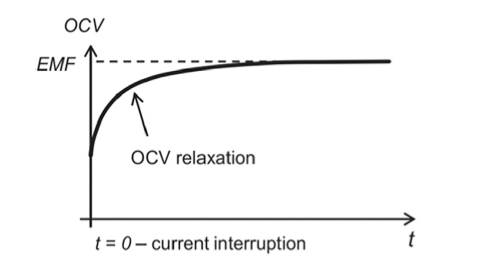
\includegraphics[width=0.7\textwidth]{EMF_Relaxation.png}
		\caption{Curva de relajación de una Batería de Li-Ion}
		\label{EMF_Method}
	\end{center}
\end{figure}


\clearpage

\subsubsection{Estimación basada en modelos (Térmico y electroquímicos)}
Este método requiere un profundo conocimiento de los fenomenos físicos y electroquímicos dentro de las baterías, como por ejemplo la concentración de electrolito, concentración de material, densidad microscópica de corriente. Esto constituye su principal desventaja ya que es complejo y la obtención de parámetros no es trivial para todo tipo de baterías.


\subsubsection{Estimación por resistencia interna}

Este método utiliza el voltage y la corriente de la batería en conjunto para determinar la resistencia interna esta. Durante breves instantes ( menores a 10 ms) se excita la batería con pulso de corriente , asumiendo que este período es lo suficientemente acotado para no que la variación de tensión sea atribuida a la resistencia interna y no a la carga/descarga de la batería la resistencia se obtendría según la formula :

\begin{figure}[h!]
	\begin{center}
		\begin{equation}
		\frac{\Delta V}{\Delta I} = R_\Omega 
		\label{Internal_resistance_EQ}
		\end{equation}	
	\end{center}
\end{figure}

 Teniendo en cuenta que si el período del pulso es mayor la medición acumula un error considerablemente mayor respecto a pulsos breves y teniendo en cuenta que este método tiene una gran precisión únicamente en valores de SOC cercanos a la descarga,debido a que varia mucho en este rango, y al bajo valor de las resistencias (del orden de los miliohm) como se muestra en la \emph{ Fig. \ref{Internal_resistance}}, extraida de \cite{hentunen}, este método no termina siendo atractivo debido a las dificultades para obtener valores precisos de SOC, generando que sea poco utilizado de manera aislada.
 
 %\cite{hentunen}
 %Time-Domain Parameter Extraction Method for
 %Thevenin-Equivalent Circuit Battery Models
 %Ari Hentunen, Member, IEEE, Teemu %Lehmuspelto, Member, IEEE, and Jussi Suomela
 %el pdf se llama hentunen2014 en la carpeta xxxx\bms\docs\Bibliography\Papers\SOC Papers
 \begin{figure}[h!]
 	\begin{center}
 		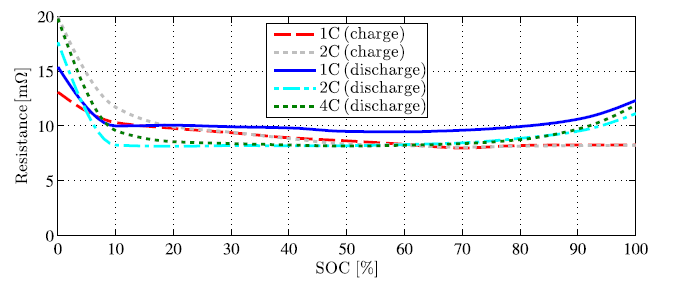
\includegraphics[width=0.7\textwidth]{Ro_vs_SOC.png}
 		\caption{Resistencia en Corriente continua de una batería de Li-Ion vs. SOC obtenida por HPPC}
 		\label{Internal_resistance}
 	\end{center}
 \end{figure}
 
 
\clearpage
\subsection{Plan de Trabajo}

Se plantea el siguiente plan de trabajo con el tiempo estimado para la finalización del proyecto:

% Please add the following required packages to your document preamble:
% \usepackage[table,xcdraw]{xcolor}
% If you use beamer only pass "xcolor=table" option, i.e. \documentclass[xcolor=table]{beamer}
\begin{table}[h!]
	\begin{tabular}{|l|c|}
		\hline
		\multicolumn{1}{|c|}{Tarea}                                                                                                                                                                              & Duración                           \\ \hline
		\begin{tabular}[c]{@{}l@{}}Estudio, análisis y comparación del estado del arte de la tecnología. \\Estudio de los requerimientos de hardware.\end{tabular}                         & 2 Semanas                          \\ \hline
		\begin{tabular}[c]{@{}l@{}}Modelado de baterías de Li-Ion en MatLab. \\Simulación de los distintos algoritmos y los circuitos de protección. \\ Estudio y comparación. Validación y elección de los más adecuados.\end{tabular} & 4 Semanas                          \\ \hline
		\begin{tabular}[c]{@{}l@{}}Desarrollo e implementación del hardware del BMS. *\end{tabular}                                                      & 6 Semanas                          \\ \hline
		\begin{tabular}[c]{@{}l@{}}Desarrollo del Firmware del BMS con los algoritmos seleccionados.\\  Implementación y depuración sobre el hardware.\end{tabular}                                                    & 4 semanas                          \\ \hline
		Montaje del banco de pruebas para ensayar las protecciones y los algoritmos correspondientes. *                                                                                                                       & 3 Semanas                          \\ \hline
		Análisis de resultados, obtención de conclusiones y desarrollo del informe final.                                                                                                                                                       & 3 Semanas                          \\ \hline
		\textbf{Total}                                                                                                                                                                                                  &\textbf{24 Semanas} \\ \hline
	\end{tabular}
\end{table}

\subsection{Extensión a futuros proyectos}

El desarrollo del hardware y los algoritmos, tanto de ecualización como de estado de carga sirven como una buena base para futuros proyectos vinculados a la temática de energías renovables y VEs.\\
\\
Como posible extensión se plantea el desarrollo de algoritmos novedosos para la estimación del Estado de Salud, su posible aplicación a sistemas de alta potencia e inclusive realizar estudios sobre nuevas tecnologías relacionadas a la composición química de las celdas.

\end{document}
